\documentclass[10pt]{article}
\usepackage[utf8]{inputenc}
\usepackage[italian]{babel}
\usepackage{multicol}
\usepackage[a4paper, total={18cm, 25cm}]{geometry}
\usepackage{listings}
\usepackage{graphicx}
\graphicspath{ {./img/} }
\begin{document}
\title{Reti di Calcolatori e Laboratorio}
\author{Federico Matteoni}
\date{ }
\renewcommand*\contentsname{Indice}

\maketitle
\tableofcontents
\pagebreak
\section{Introduzione}
Appunti del corso di \textbf{Reti di Calcolatori} presi a lezione da \textbf{Federico Matteoni}.\\\\
Prof.: \textbf{Federica Paganelli}, federica.paganelli@unipi.it\\
\begin{list}{-}{Riferimenti web:}
\item \emph{elearning.di.unipi.it/enrol/index.php?id=169}\\Password: \textbf{RETI2019}
\end{list}
Esame: scritto (o compitini), discussione orale facoltativa + progetto con discussione (progetto + teoria di laboratorio, progetto da consegnare 7gg prima della discussione)\\
\begin{list}{-}{Libri e materiale didattico:}
\item Slide su eLearning
\item IETF RFC\\tools.ietf.org/rfc\\www.ietf.org/rfc.html
\item "Computer Networks: A Top-Down Approach" B. A. Forouzan, F. Mosharraf, McGraw Hill
\end{list}
Ricevimento: stanza 355 DO, II piano

\section{Rete}
\paragraph{Definizione di rete} Interconnessione di dispositivi in grado di scambiarsi informazioni, come end system, router, switch e modem.\\
\begin{list}{}{Gli end system possono essere di due tipi:}
\item \textbf{Host}: una macchina, in genere di proprietà degli utenti, \textbf{dedicata ad eseguire applicazioni}. Esempi: desktop, portatile, smartphone, tablet\ldots
\item \textbf{Server}: una macchina, tipicamente con elevate prestazioni, destinata ad eseguire programmi che \textbf{forniscono servizi} a diverse applicazioni utente. Esempi: posta elettronica, web, \ldots
\end{list}
\textbf{Con il termine host si può anche indicare un server}.

\subsection{Tipi di Rete}
\paragraph{Local Area Network} Una \textbf{LAN è una rete di area geografica limitata}: un ufficio, una casa ecc.. I dispositivi comunicano attraverso una determinata tecnologica: switch, BUS, HUB ecc..\\
In una rete locale tipicamente una serie di host comunicano tra loro attraverso, ad esempio, uno switch centrale.
\paragraph{Wide Area Network} Alcuni esempi:\\
\begin{multicols}{2}
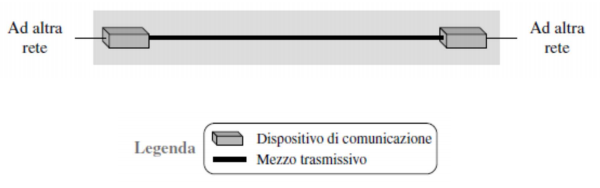
\includegraphics[scale=0.5]{wan1.png}\\
\columnbreak
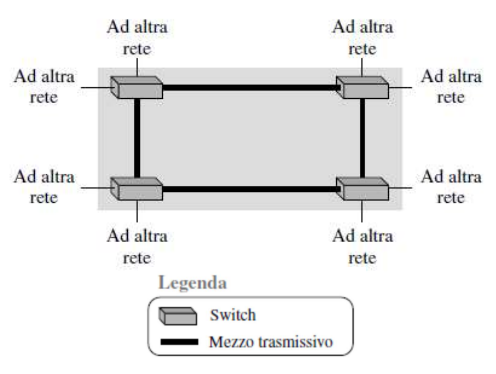
\includegraphics[scale=0.5]{wan2.png}\\
\end{multicols}

\subsection{Internetwork}
Una \textbf{internetwork} si crea quando si \textbf{interconnettono diverse reti}.
Alcuni esempi:\\
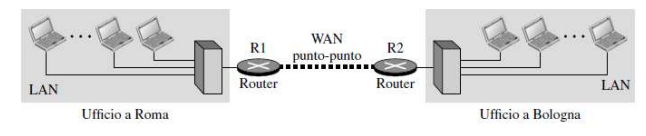
\includegraphics[scale=1]{internetwork1.png}\\
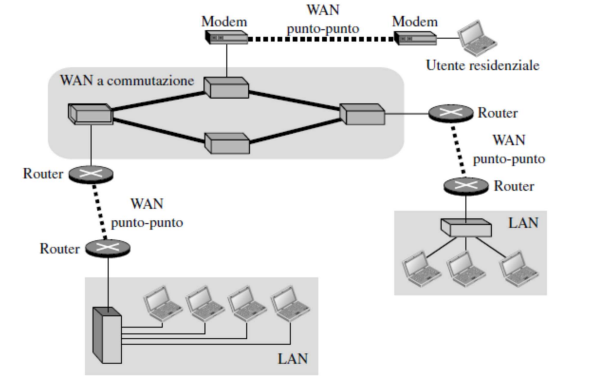
\includegraphics[scale=0.75]{internetwork2.png}\\

\subsection{Switching}
Una rete internet è formata dall'interconnesione di reti composte da link e dispositivi capaci di scambiarsi informazioni.
In particolare, i sistemi terminali comunicano tra di loro per mezzo di dispositivi come switch, router ecc. che si trovano nel percorso tra i sistemi sorgente e destinazione.
\paragraph{Switched Network} Reti a commutazione di circuito, tipico delle vecchie reti telefoniche\\
Le risorse sono riservate end-to-end per una connessione. Le risorse di rete (es. bandwidth) vengono suddivise in pezzi, e ciascun pezzo è allocato ai vari collegamenti. Le risorse rimangono inattive se non vengono utilizzate, cioè \textbf{non c'è condivisione}. L'allocazione della rete rende necessario un setup della comunicazione.\\A tutti gli effetti vi è un circuito dedicato per tutta la durata della connessione. Ciò è rende poco flessibile l'utilizzo delle risorse (\textbf{overprovisioning}).
\paragraph{Packet-Switched Network} Reti a commutazione di pacchetto, più moderno\\
Flusso di dati punto-punto suddiviso in pacchetti. I pacchetti degli utenti condividono le risorse di rete. Ciascun pacchetto utilizza completamente il canale.\\\textbf{Store and Forward}: il commutatore deve ricevere l'intero pacchetto prima di ritrasmetterlo in uscita.\\Le risorse vengono usate \textbf{a seconda delle necessità}. Vi è \textbf{contesa per le risorse}: la richiesta di risorse può eccedere la disponibilità e si può verificare \textbf{congestione} quando i pacchetti vengono accodati in attesa di utilizzare il collegamento. Si possono anche verificare perdite.
\section{Internet} L'internetwork più famosa ed utilizzata è \textbf{internet}, ed è composta da migliaia di reti interconnesse. \textbf{Ogni rete} connessa ad internet \textbf{deve utilizzare il protocollo IP} e rispettare certe convenzioni su nomi ed indirizzi. Si possono aggiungere nuove reti ad internet molto facilmente.
\paragraph{Dispositivi in internet} I \textbf{dispositivi} connessi ad internet possono essere host, end systems come PC, workstations, servers, pda, smartphones ecc\ldots\\
I \textbf{link di comunicazione} possono essere fibre ottiche, doppini telefonici, cavi coassiali, onde radio\ldots
Le \textbf{entità software} in internet possono essere:
\begin{list}{}{}
\item \textbf{Applicazioni} e processi
\item \textbf{Protocolli}: regolamentano la trasmissione e la ricezione di messaggi (TCP, IP, HTTP, FTP, PPP\ldots)
\item \textbf{Interfacce}
\item \textbf{Standard} di internet e del web: RFC (Request for Comments) e W3C.
\end{list}
\textbf{Internet è una visione dei servizi}. L'infrastruttura di comunicazione permette alle applicazioni distribuite di scambiare informazioni (WWW, e-mail, giochi, e-commerce, controllo remoto\ldots) e fornisce loro \textbf{servizi di comunicazione connectionless} (senza garanzia di consegna) o \textbf{connection-oriented} (dati garantiti in integrità, completezza ed ordine).
\subsection{Enti Ufficiali} L'\textbf{Internet Engineering Task Force} (IETF) è l'organismo che studia e sviluppa i protocolli in uso su internet. Si basa su gruppi di lavoro a cui chiunque può accedere. I documenti ufficiali che pubblica, dove descrivono i protocolli usati in internet, sono gli RFC/STD (Request for Comments/STanDards).\\
L'\textbf{Internet Corporation for Assigned Names and Numbers} (ICANN) si occupa di coordinare il sistema dei \textbf{nomi di dominio} (DNS) e assegna i gruppi di indirizzi, gli identificativi di protocollo.\\\\
\begin{center}
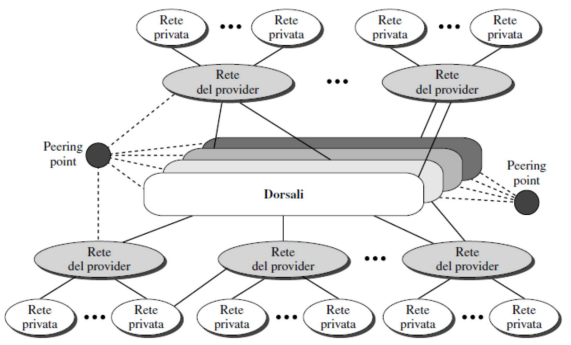
\includegraphics[scale=1]{internet.png}\\
\textbf{Peering point}: interconnessione tra due sistemi autonomi\\
\end{center}
\pagebreak
\subsection{Reti di accesso} Il collegamento tra l'utente ed il primo router di internet è detto \textbf{rete di accesso}.
\begin{list}{}{Può avvenire in 3 modi:}
\item \textbf{Tramite rete telefonica}: servizio dial-up, ADSL\ldots
\item \textbf{Tramite reti wireless}
\item \textbf{Collegamento diretto}, come collegamenti WAN dedicati ad alta velocità (aziende e università)
\end{list}
\section{Metriche di Riferimento}
Come misurare le prestazioni della rete?
\begin{list}{}{Tramite una serie di metriche:}
\item \textbf{Bandwith} o ampiezza di banda: è la larghezza dell'intervallo di frequenze utilizzato dal sistema trasmissivo (Hz).\\\textbf{Bitrate} o \textbf{transmission rate}: quantità di bit che possono essere trasmessi o ricevuti nell'unità di tempo (bit/secondo, bps)\\Il bitrate dipende dalla bandwidth e dalla tecnica trasmissiva utilizzata.
\item \textbf{Throughput}: la quantità di traffico che arriva realmente a destinazione nell'unità di tempo (al netto di perdite sulla rete, funzionamento dei protocolli ecc\ldots).\\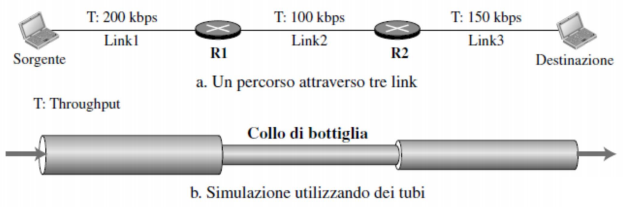
\includegraphics[scale=1]{throughput.png}\\Non è detto che corrisponda alla bandwidth perché ci potrebbe essere un collo di bottiglia.
\item \textbf{Latenza} o ritardo: il tempo richiesto affinché un messaggio arrivi a destinazione dal momento in cui il primo bit parte dalla sorgente.\\
\texttt{latenza = ritardo di propagazione + ritardo di trasmissione + ritardo di accodamento + ritardo di elaborazione}
\item \textbf{Perdita di pacchetti}. Come si può verificare?\\
\begin{multicols}{2}
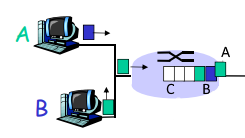
\includegraphics[scale=1]{ritpackets.png}\\

\columnbreak
A $\rightarrow$ pacchetti \textbf{in attesa} di essere trasmessi (\emph{ritardo})\\
B $\rightarrow$ pacchetti \textbf{accodati} (\emph{ritardo})\\
C $\rightarrow$ buffer \textbf{liberi} (se non ci sono buffer liberi, i pacchetti in arrivo vengono scartati, \emph{perdita})\\\\
I pacchetti da spedire vengono accodati nei buffer dei router. Di solito, il tasso di arrivo dei pacchetti sul router eccede le capacità del router di evaderli, quindi \textbf{i pacchetti si accodano in attesa del proprio turno}.
\end{multicols}
Il \textbf{ritardo di elaborazione} è dato dal controllo sui bit e dalla determinazione del canale di uscita (trascurabile)\\
Il \textbf{ritardo di accodamento} è dato dall'attesa di un pacchetto di essere trasmesso (B)\\
Il \textbf{ritardo di trasmissione} è il tempo impiegato per trasmettere un pacchetto sul link.\\\texttt{R$_{trasmissione}$ = R/L}\\
\texttt{R} = rate di trasmissione del collegamento, in bps\\
\texttt{L} = lunghezza del pacchetto in bit\\
Il \textbf{ritardo di propagazione} è il tempo impiegato da 1 bit per essere propagato da un nodo all'altro.\\\texttt{R$_{propagazione}$ = d/s}\\
\texttt{d} = lunghezza del collegamento\\
\texttt{s} = velocità di propagazione del collegamento (si usa la velocità della luce, circa 3 x 10$^{8}$ m/s)
\end{list}
\texttt{d$_{nodal}$ = d$_{proc}$ + d$_{queue}$ + d$_{trans}$ + d$_{prop}$}\\
\texttt{d$_{proc}$} = \textbf{ritardo di elaborazione}, pochi microsecondi\\
\texttt{d$_{queue}$} = \textbf{ritardo di accodamento}, dipende dalla congestione\\
\texttt{d$_{trans}$} = \textbf{ritardo di trasmissione}, \texttt{L/R} e significativo a lunga distanza\\
\texttt{d$_{prop}$} = \textbf{ritardo di propagazione}, \texttt{d/s}, da pochi microsecondi a centinaia di millisecondi\\
\section{Modelli Stratificati}
$https://elearning.di.unipi.it/pluginfile.php/27387/mod_resource/content/1/L02_introduzione_protocolli.pdf$
\paragraph{Perché un modello a strati} Per mandare dati da un host all'altro comunicando su rete si devono eseguire una serie di operazioni: \textbf{trovare il percorso} di rete da attraversare, \textbf{decidere in che modo spedire e codificare} i dati, \textbf{risolvere eventuali problemi} di comunicazione e altro ancora. Programmare ogni volta tutto il procedimento è un lavoro estremamente complesso e ripetitivo. Il modello a strati \textbf{astrae su più livelli il problema della trasmissione dati} in modo da fornire di volta in volta strumenti al programmatore per poter evitare di "\textit{reinventare la ruota}".
\paragraph{Definizioni generali} Nelle architetture di comunicazione a strati sono importanti una serie di definizioni:
\begin{list}{-}{}
\item Stratificazione
\item Information hiding
\item Separation of concern
\item Modello ISO/OSI
\item Stack TCP/IP
\end{list}
Tali definizioni verranno viste durante il corso.

--roba simone--

\subsection{Protocollo}
\paragraph{Cos'è un protocollo} insieme di regole che dice come comunicare ed esporre verso l'esterno.
\paragraph{Es. modello stratificato: sistema postale} vedi slide, da livello alto a livello basso per spedizione, viceversa per ricevere (da basso ad alto). Il problema grosso di mandare lettera in ita a jap in una serie di passi, in cui viene eseguito un particolare compito su un messaggio, che viene trasferito ad un altro livello. Segretaria prepara lettera affinché postino la possa prendere. Però il messaggio scritto da un livello è pensato per essere interpretato dallo stesso livello del sistema di arrivo (segretaria scrive per segretaria, direttore scrive per direttore).
\subsection{Incapsulamento} aggiungo strati, involucri al messaggio originale che vengono man mano tolti alla destinazione.
\subsection{Perché stratificare} prendo sistema che per una singola coppia di aziende è costoso, lo trasformo a strati così che il costo della singola lettera sia irrisorio.
Definisco funzioni di base per effettuare trasferimento e agenti che le svolgono.
Principi di base: separation of concern e information hiding
\subsubsection{Separation of Concern}
Fare ciò che compete delegando agli altri ciò che è delegabile.
\subsubsection{Information Hiding}
Nascondere info non indispensabili affinché il committente possa svolgere l'operazione.

se traduco modlelo postale in a strati ho\\
utente\\segretaria\\postino\\smistamento\\stazione\\
smistamento intermedio: arrivo fino ad un livello intermedio per evitare che si possano esporre info sensibili.\\\\
vantaggi a strati: svilupp e impl singolo strato più semplice rispetto a fare tutto il complesso\\
servizi di strati inferiori usati da più entità di strati superiori\\\\
\subsection{OSI RM (Open Systems Interconnction Reference Model)}
Prime reti chiuse, tecnologie e protocolli proprietari. Es. ARPANET, SNA (IBM), Dna (Digital), non intercomunicavano. Le reti erano per servizi specifici (TELCO)\\
Quindi obiettivo: modello riferimento per sistemi aprti (quasliasi terminale deve poter comunicarer mediante qualsiasi rete). $\rightarrow$ accordarsi sulle regole\\\\
OSI era un set di protocolli aperti: dettagli pubblici e cambiamenti gestiti da organizzazione con partecipazione aperta al pubblico. Un sistema che implementa protocolli aperti è un sistema aperto. L'ISO.\\
Elementi fondamentali modello stratificiato:\\
flusso dati\\servizi\\protocolli\\interfacce\\
uno strato fornisce servizi a strato sopra e richiede servizi a strato sotto. Strato n comunica con strato n di altra unità tramite protocollo assegnato. comunicaz strati attraverso interfaccia.\\

\subsection{Protocolli}
\paragraph{cos'è un protocollo (x2)} protocolli definiscono formatop e ordine messaggi inviati e ricevute e azioni per trasmette e ricevere messaggi.
\subparagraph{efficace} sistema raggiunge socpo con maggior freq possibile
\subparagraph{efficiente} sistema raggiunge scopo con minor sforzo possibile

\subsubsection{Pila di protocolli}
OSI prevede sette strati\\
7-5 più modi di raggrupparli, livello software e applicativo\\
7 applicativo: elaborazione dati\\
6 presentazione: unificazione dati, preparazione del pacchetto\\
5 sessione: controllo del dialogo tra due host sorgente e dest. Decidere regole per la comunicazione tra due host.\\
4 trasporto: offre trasferimento dati tra host terminali. Astrazione logica per cui si consegna a questo livello un messaggio e dove mandarlo. \textbf{dialogo end-to-end}\\
3 rete: instradamento del traffico (router, offre il servizio di consegna attraverso sistema distribuito di nodi intermedi)\\
2 datalink: frame fra interfacce, scheda di rete deve interpretare il flusso di bit\\
1 fisico: mezzo fisico, modulare segnale elettrico per trasmettere il flusso di bit\\
4-1 livelli fisico+sw\\\\
servizio: funzione che uno strato offre a strato superiore, attraverso un'interfaccia\\
interfaccia: regole che governano formato e significato frame, pacchetti o messaggi che vengono scmabiati tra strati successivi della stessa entità\\
servizi cosa, interfaccia come\\\\
connection-oriented: livello trasferimento crea connessione logica tra due sistemi (instaurazione connessione, trasferimento dati, chiusura connesione)\\
connectionless: dati trasmessi senza stabilire connessione\\

\section{Flusso dell'Informazione}
Qualcuno (livello applicativo) genera dati da mandare in remoto. L'info scende i livelli fino al canale fisico, e ogni livello aggiungeall'informazione ricevuta dal livello superiore una propria (o più) sezione informativa sotto forma di header con info esclusive di quel livello.\\
HEADER|DATA|TRAILER\\
header: qualificazione del pacchetto per questo livello\\
data: payload dal liv superiore\\
trailer: coda\\
slide esempio incapsulamento dei dati\\

\section{Stack protocollare TCP/IP}
famiglia protocollo attualmente usati in interneti. gerarchia di protocollli costituita da moduli interagenti ciascuno ocn funz specifiche.\\
gerarchia: ciascun protocollo liv superiore è supportato da servizi di livelli inferiore\\\\
applicaizone: supporta applicazione rete: smtp, ftp, http\\
trasporto: trasferimento dati host-host: tcp, udp\\
rete: instradamento datagrammi dalla sorgente alla destinazione e protocolli di management rete: ip, icmp\\
link: trasferimento dati tra elementi di rete vicini (da un hop all'altro): ppp, ethernet,... qualunque cosa\\
fisico: aggiunto successivamente: bits on the wire\\\\
come protocollo la specifica fa comuniazione a livello orizzontale (da livello n origine a livello n destinazione).\\
\paragraph{Livello Applicativo} Il livello più alto, con il quale interagisce l'utente\\
Identificativi risorse: URL, URI, URN\\
Il web: user agents, http: request, response, connessioni persistenti, GET, POST, PUT, DELETE, status code, proxy server, caching\\
FTP: connessioni dati e di controllo, rappresentazione\\
TELNET\\
Posta elettronica: SMTP, POP3, IMAP\\
DNS e risoluzioni nomi: gerarchia nomi, risoluzione iterativa e ricorsiva, formato pessaggi, nslookup...\\
\paragraph{Livello Trasporto} Livello al quale si definisce la codifica e il protocollo di trasporto\\
Servizi: mux demux, co ntrollo errore, connectionless\\
TCP: formato segmenti, gestione connessione, controllo flusso e congestione\\
UDP: formato segmenti\\
\paragraph{Livello Rete} Dove si gestisce l'indirizzamento dei vari host\\
strato di rete e funzioni\\
indirizzamentoi ip: classful IPv4, NAT, sottoreti e maschere, classless, CIDR\\
risoluzione IP e MAC, ARP\\
IPv4: formato datagramma ip, frammentazione\\
routing IP e istradamento\\
introduzione IPv6\\
\paragraph{Link} Il livello più basso, dove avviene la vera e propria comunicazione a livello elettrico\\
Cenni livello link\\
Ethernet\\
\subsection{strato applicativo}
$https://elearning.di.unipi.it/pluginfile.php/27477/mod_resource/content/2/L03_Applicativo_HTTP.pdf$
\end{document}